\documentclass[a4paper,12pt]{article}
\usepackage[utf8]{inputenc}
\usepackage[T1]{fontenc}
\usepackage[slovene]{babel}
\usepackage{graphicx}
\graphicspath{{./Slike/}}
\usepackage{amsmath}
\usepackage[colorinlistoftodos]{todonotes}

\title{Problem iskanja najdaljšega drevesa v ravnini}

\author{Ema Kozin in Filip Škrlj}

\date{december in januar 2020}

\begin{document}
	
\maketitle
	
\newpage

\tableofcontents
	
\newpage
\section{Prestavitev problema}

Pogledala sva si, kako bi na dani množici $P$, ki vsebuje $n$ točk, našla graf z največjo dolžino, za katerega velja, da se njegove povezave ne križajo ter je drevo.
 Problem bova prikazala na nekaj primerih in ugotovila, v kolikšen času, je ta problem rešljiv glede na velikost množice $P$. 


\section{Algoritem}

\subsection{Opis}
Pri reševanju problema se bova osredotočila na iskanje najdaljše \emph{dvozvezde}, torej drevesa s takima točkama $a$ in $b$,
 da v tem drevesu obstaja povezava med njima
in da je vsaka druga točka povezana bodisi z $a$ bodisi z $b$. Sedaj lahko uporabimo dinamično programiranje. \\
Brez škode za splošno lahko predpostavimo, da $a$ leži levo od $b$, ti točki naj ležita na vodoravni črti, nad katero so še vse preostale točke. \\
Naprej si ogledamo podproblem, označen s parom $(p, q)$ , kjer sta $p$ in $q$ iz množice $P$ in se povezavi $ap$ in $bq$ ne sekata.
 Za vsak tak par $(p, q)$ opazimo, da povezave $ap, pq, qb$ in $ba$ tvorijo štirikotnik. Naj bo sedaj z $Q(p,q)$ označen del tega štirikotnika, ki je pod črto,
  vzporedno stranici $ab$, ki gre skozi nižje ležečo točko izmed $p$ in $q$, torej pod $y = min\{y(p),y(q)\}$. Glej spodnjo sliko.\\
  
\begin{figure*}[h]
	\centering
	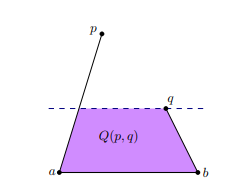
\includegraphics{primer_Q(p,q).png}
\end{figure*}


Dolžino najdaljše dvozvezde s korenoma $a$ in $b$ na točkah znotraj $Q(p,q)$ označimo z $Z(p,q)$, 
pri tem pa ne upoštevamo dolžine povezave $ab$. Če $Q(p,q)$ ne vsebuje nobene točke iz $P$, je $Z(p,q) = 0$. \\
V primeru, da vsebuje vsaj eno točko iz $P$, pa označimo s $k_{p,q}$ najvišje ležečo točko znotraj $Q(p,q)$. 
To točko povežemo z točko $a$ ali točko $b$. Če jo povežemo z $a$, bomo tudi točke, 
ki so znotraj trikotnika $L_{p,q}$, omejenega z povezavama $ap$ in $ak_{p,q}$ in vodoravno črto $y = y(k_{p,q})$ ,
 povezali z $a$. Podobno, če $k_{p,q}$ povežemo z $b$, dobimo trikotnik na desni strani, označen z $R(p,q)$, omejen z $bq,bk_{p,q}$ in $y=y(k_{p,q})$. \\
 
 \begin{figure*}[h]
 	\centering
 	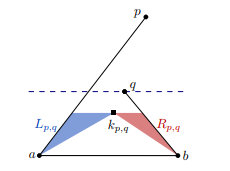
\includegraphics{trikotnika.png}
 \end{figure*}

V prvem primeru dobimo namesto para $(p,q)$ nov par $(k_{p,q}q)$, v drugem primeru pa par $(p,k_{p,q})$. Za vsak veljaven par $(p,q)$ dobimo naslednje:
\begin{equation*}
		$$\[ Z(p,q) = \left\{ \begin{array}{ll}
			0 & \mbox{če v $Q(p,q)$ ni točke iz $P$};\\
			max \left\{ \begin{tabular}{ccc}
				$Z(k_{p,q},q) + \|ak_{p,q} \| + \sum_{l \in L_{p,q}}\|al\| $ \\
				$Z(p, k_{p,q}) + \|bk_{p,q}\| + \sum_{r \in R_{p,q}}\|br\| $
			\end{tabular} \right\} & \mbox{sicer}\end{array} \right. \]$$
\end{equation*}
Zgornjo zvezo bova uporabila na vsakem veljavnem paru $(p,q)$ in tako našla najdaljšo dvozvezdo s korenoma $a$ in $b$.

\subsection{Koda}

Najino kodo za reševanje problema iskanja najdaljšega drevesa sva uporabila programski jezik \emph{Python}.
  Koda z komentarji je vsebovana v datoteki \emph{$ogrodje\_in\_algoritem.py$} na najinem repozitoriju.
   V tem poročilo pa bova opisala njene glavne komponente, ključne za rešitev problema.Glavni del kode sva razdelila na tri dele, funkcije \emph{pomožna, pomožna\_B in algo}. \\
Funkcija \emph{pomožna} sprejme naslednje argumente: naš graf ter točke $a, b, p$ in $q$ (v opisu algoritma sva že razložila njihovo uporabo in pomen).
 Funkcija najprej preveri, ali ima par $(p, q)$ že določeno vrednost $Z(p,q)$, 
 ki predstavlja dolžino najdaljše dvozvezde s korenoma v $a$ in $b$. Potem določimo štirikotnik $Q(p,q)$ tako, 
 da primerjamo razdalji med daljico $ab$ in točkama $p$ in $q$. 
 Nato najdemo še točko znotraj tega štirikotnika, ki je najdlje od daljice $ab$ in jo označimo z $k$.
  Definiramo še levi trikotnik (če $k$ povežemo z $a$) in desni trikotnik (če $k$ povežemo z $b$). 
  Če je znotraj teh trikotnikov še kakšna druga točka našega grafa, jo povežemo z ustrezno točko izmed $a$ in $b$.
   V primeru levega trikotnika nadaljujemo naš postopek z novim parom $(k,q)$, v primeru desnega pa z parom $(p, k)$.
    Na koncu vse združimo in z uporabo naše formule iz opisa algoritma izračunamo $Z(p,q)$ za štirico točk $(a, b, p, q)$. \\
Naslednja pomemnba funkcija je \emph{pomožna\_B}, ki funkcijo \emph{pomožna} uporabi na vseh parih $(p,q)$ našega grafa.
 Najprej preveri, koliko je točk v grafu. Če sta točki le dve, torej ravno $a$ in $b$, je naša dvozvezda dolžine $0$. 
 Če so točki tri, pa je dolžina najdaljše dvozvezde enaka maksimalni dolžini med točko $a$ oziroma točko $b$ in tretjo točko.
  Ko pa je točk več, funkcija preveri s pomočjo funkcije \emph{alisesekata}, ali je par točk,
   ki bi ju radi povezali z $a$ in $b$ primeren in nato v tem primeru uporabi funkcijo \emph{pomožna}. \\
Nazadnje funkcija \emph{algo} steče po vseh točkah grafa, jih uporabi za korena dvozvede $a$ in $b$ 
ter naprej uporabi funkcijo \emph{pomožna\_B} na ta kandidata korenov. 
Za vsak tak par korenov preveri, če je njuna dvozvedza najdaljša in na koncu to najdaljšo dolžino izpiše. 

\section{Sklep}

Z uporabo najine kode sva ugotovila, da je problem res rešljiv v času $O(n^2)$ preko dinamičnega programiranja kot je sugerirala najina literatura. Pri primerih uporabe kode na kvadratu, ozkem pravokotniku in kolobarju sva to potrdila. 

\newpage

\begin{thebibliography}{5}
	\bibitem{1}
	Sergio Cabello, Michael Hoffmann, Katharina Klost, Wolfgang Mulzer, Josef Tkadlec. \textit{Long plane trees (work in progress)}
	\bibitem{2}
	Ahmad Biniaz, Prosenjit Bose, Kimberly Crosbie, Jean-Lou De Carufel, David Eppstein, Anil Maheshwari, Michiel Smid. \textit{maximum plane trees in multipartite geometric graphs. Algorithmica}
	\bibitem{3}
	Noga Alon, Sridhar Rajagopalan, Subhash Suri. \textit{Long non-crossing configurations in the plane. Fundam.}
\end{thebibliography}


	
\end{document}